\section{Практическая часть}

Расчет распределения Пуассона выводится с помощью функции POISSON(RNj, $\lambda$), где RNj --- означает  порядковый номер датчика случайной величины, обычно от 1 до 7; $\lambda$ --- параметр.

В листинге 3.1 представлена реализация системы массового обслуживания на языке имитационного моделирования GPSS.

\begin{lstlisting}[caption=Реализация системы массового обслуживания]
	GENERATE (UNIFORM(1,1,5)),,,1000
	Enqueue QUEUE QSystemQueue
	
	SEIZE Operator
	DEPART QSystemQueue
	
	ADVANCE(POISSON(1,9))
	RELEASE Operator
	
	TRANSFER 0.7,Complete,Enqueue 
	Complete TERMINATE 1
	
	START 1000
\end{lstlisting}

\clearpage

На рисунке 3.1 демонстрируется работа программы. Максимальная длина очереди при вероятности возврата заявки 0.7 равна 811 заявки.

\begin{figure}[h]
	\centering
	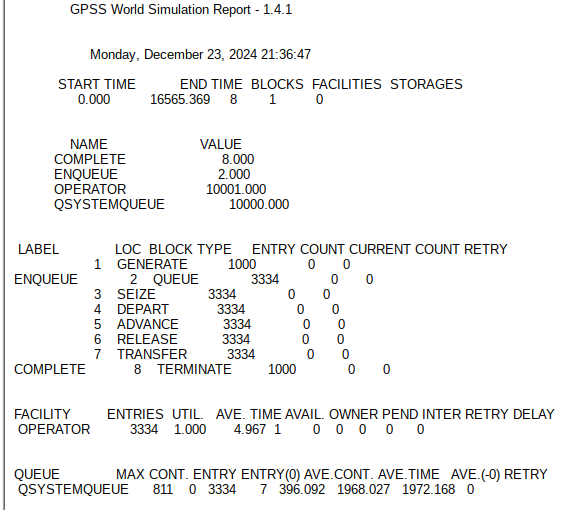
\includegraphics[height=0.55\textheight]{../img/res.png}
	\caption{Отчёт системы массового обслуживания}
	\label{plt:even_comp_alg}
\end{figure}

